\documentclass[twocolumn,12pt]{article}
\usepackage{tikz}
\usetikzlibrary{calc}
\newcommand{\tikzmark}[1]{\tikz[overlay,remember picture] \node (#1) {};}
\newcommand{\underarrow}[2] {
  \begin{tikzpicture}[overlay,remember picture,out=340,in=210,distance=0.3cm]
    \draw [->,shorten >=3pt,shorten <=-3pt] ({#1}.south) to ({#2}.west);
  \end{tikzpicture}
}  
\newcommand{\Ex}{\mathbb{E}}
\usepackage{graphicx}
\usepackage{dblfloatfix}
\usepackage[superscript,biblabel]{cite}
\usepackage{multirow,tabularx}
\usepackage{hhline}
\usepackage{amsmath}
\usepackage[margin=1in]{geometry}
\usepackage{cancel}

\newcommand\indep{\protect\mathpalette{\protect\independenT}{\perp}}
\def\independenT#1#2{\mathrel{\rlap{$#1#2$}\mkern2mu{#1#2}}}

\title{Inferring Causality from Finite Data using Conditional Independence}
\author{Daniel Speyer}
%\address{dls2192@columbia.edu}
\begin{document}

\maketitle

\begin{abstract}
  There exist many techniques for inferring causal structure from
  conditional independence, but they all assume establishing
  conditional independence is trivial, which from a finite sample it
  is not.  Also, all return a graph,
  rather than a graph and a probability that it is the correct one.
  In this paper I offer two techniques of limited scope that address
  these problems.  I then discuss the techniques limitations, and
  apply them to finding probiotic treatments for Crohn's Disease.
\end{abstract}

\section{Introduction}

Inferring causal graphs from observational data is a widely-sought
goal in statistics.  The most common tool for it is conditional
independence.  The specifics of a causal graph determine which node
are independent conditioned on which others by the ``bayes ball''
rule, and therefore it should be possible to observe the independences
and work backward to the causal graph.

This has proved to be more difficult in practice.  In particular,
observing independence is not as simple as it sounds.  Pearl suggests
we test joint conditional probability distributions for equality\cite{Pearl}.
Leaving aside the curse of dimensionality, this assumes we have the
exact distributions.  If all we have is a finite random sample from
those distributions, we can construct posteriors, but we cannot perform
an equality test.  Spirtes, Glymour and Shine  encourage us to assume that
``the statistical decisions required by the [causal inference]
algorithms are correct
for the population'', while admitting that this ``is often not met in
practice''\cite{Spirtes}.  Others have described this as ``possessing an
independence oracle''\cite{Peters,pcalg}.  Many simply include a ``test if $a\indep
b|s$'' step in their algorithms, assuming the reader will already know
how.

In practice, the usual solution is to treat independence as a null
hypothesis, try to reject it at some p threshold, and treat any
failure as establishing it.  Needless to say, this is incorrect.

Dealing with finite data means the possibility of dealing with too
little data.  The elegant solution is to give some numerical
expression of confidence which becomes ``I don't know'' when the data
gets too small.  This solution has another benefit: in the biomedical
context, it is routine to test thousands of equally plausible
hypotheses at once.  A flat accuracy of 99\% is unhelpful in the face
of this, but a numeric expression of confidence allows proper
compensation.

\subsection{Motivating Problem: Crohn's Disease}

This paper is optimized around a specific practical problem:
untangling the microbiome's role in Illial Crohn's Disease.  It is
well established that there are many differences in the intestinal
bacteria of healthy people and of people with the disease\cite{hofer}, but it is
not established whether the differences of bacteria \textit{cause} the
disease.  If we can find a set of bacteria such that
p(disease $|$ do(bacteria)) is low, we will have a cure for the disease.
There have been attempts to determine this by randomized controlled
trial, but early results are discouraging\cite{rctma} and the number
of species, combined with other relevant
variables, make exhaustive RCTs impractical.

Data is available on this problem\cite{data}, including genetic, microbiome and
health information, but for only 58 patients.  The microbiome
information is a series of 16S reads, but can generally be described
as ``present'' or ``absent'', with very low concentrations of a
species rounded off to ``absent''.  This comes much closer to fitting
the empirical distributions than any convenient scalar formula, which
is why this paper will use binary variables.

\section{Extending Graphs}

Let us begin with the simplest case.  Suppose we have a known cause, a
known effect, and a variable which connects to the effect in an
unknown way, that is $A \rightarrow B$ -- $C$.  We do not observe a
correlation between $A$ and $C$, but that might only mean our test is
underpowered.  For Crohn's Disease, $A$ would be mutations in the NOD2
gene\cite{nod2}, $B$ would be the disease, and $C$ would be each of 222
species of plausibly relevant bacteria.

For now, we will assume that there is no direct causal
link between $A$ and $C$, and furthermore that there are no unobserved
confounders or selection effects.  We will consider these later.
This leaves us only two models, $A \rightarrow B \rightarrow C$ or $A
\rightarrow B \leftarrow C$.  We can call these ``chain'' and
``collide'' models, or $m_{ch}$ and $m_{co}$ for short.  Can we
distinguish between them?

Yes.  Let us consider
$p(A,C)$:

\begin{eqnarray*}
p(A,C|m_{ch}) & = & \sum_B p(A)p(B|A)p(C|B) \\
p(A,C|m_{co}) & = & p(A)p(C)
\end{eqnarray*}

We do not actually know the terms on the right side of those
equations, so let us parameterize both models with $\theta$ and
rewrite the equations as:


\begin{multline*}
  p(A,C|m_{ch}) = \\
  \int \left ( \sum_B p(A|\theta) p(B|A,\theta) 
  p(C|B,\theta) \right ) p(\theta) d\theta \\
  p(A,C|m_{co}) = \int p(A|\theta)p(C|\theta)p(\theta) d\theta
\end{multline*}

We can learn $p(\theta)$ from available data using dirichlet priors.
The integrals would be difficult algebraically, but they can be
adequately approximated with monte-carlo sampling.

Once we have these, let $n_{a,c}$ be the count of datapoints with
A=a,C=c and we can use:

\begin{equation*}
p(n_*|m) \propto \prod_{a,c} p(a,c|m)^{n_{a,c}}
\end{equation*}

Proportional instead of equal because there is a combinatoric term,
but it cancels when taking odds ratios so it can be safely ignored.

From here, we can apply standard bayesian updating.  Empirically, this
works well.  With all probabilities chosen at random, the mean log
probability it assigns to the wrong model is only -0.62.  Furthermore,
if the output is bucketed by posterior, the fraction correct forms a
graph very similar to a straight line (see figure \ref{dir_pla58}).
It does show a minor bias toward chain models, but it goes away at the
edges, and collider models are the useful ones, so this is a safe bias.

While the test is well-calibrated, it returns bayes factors very close
to one most of the time.  For random probabilities and 58 datapoints,
it only gives a clear answer (i.e. a bayes factor outside the range
[0.1,10] 8\% of the time).  This includes cases in which one of the
causal effects is very weak.  Altering the generative function to more
closely resemble the Crohn's data (by having the real p(NOD2) and
p(Crohn's$|$NOD2) and detectable $B\not\indep C$) brings this up to
13\%.  Even with realistic data, 500 datapoints are needed to gain
conclusive answers more than half the time (see figure
\ref{dir_use}).  The realistic data does make the test somewhat less
calibrated (figure \ref{dir_crohns58}), which probably reflects a
collide model being more likely to produce Crohns-like data in the
first place, but the errors remain small and on the side of safety.

\subsection{Non-Simply-Connected Graphs}

What if there is a causal effect $A\rightarrow C$?  It must be weak
enough not to be detected, but that doesn't say much.  Let us consider
it by cases.

\subsubsection{False Colliders}

Can a true graph of
$A\tikzmark{a}\rightarrow B \rightarrow{C}\tikzmark{c}$
\underarrow{a}{c}
produce a $p(A,C)$ more similar to a graph
$A \rightarrow B \leftarrow C$?  This would require the direct and
indirect influence of $A$ on $C$ to cancel out rather precisely.  If
the indirect influence is stronger, we will pick the correct model,
albeit underconfidently.  If the direct influence is too strong, we
will see a correlation between $A$ and $C$.  And if the direct
influence is in the same direction as the indirect, the correct model
will remain the better fit (though both models will be worse).

\subsubsection{False Chains}

Similarly, can a true graph of
$A\tikzmark{a2}\rightarrow B \leftarrow{C}\tikzmark{c2}$
\underarrow{a2}{c2}
produce a $p(A,C)$ more similar to a graph
$A \rightarrow B \rightarrow C$?  Again, this is possible, but there
is no reason for $p(C|A)$ to resemble $\sum_B p(B|A)p(C|B)$.  If
$p(C|A)-p(C|\bar{A})$ is too large, $A\not\indep C$ will be detected
initially, whereas if it's too small, the correct model will be
chosen.  Furthermore, what shrinks the upper bound is for the
predicted A-C relation in the chain model to be small, which also
means any erroneous bayes factor will be small.

\subsubsection{Empirical Examination}

These examinations are difficult to make rigorous, but simulation
suggests there is little to worry about.  If an $A\rightarrow C$ link
is added but bounded by a $\chi^2$ test, there is a tendency toward
underconfidence, but little other effect (see figure
\ref{dir_multi58}.  This applies to the Crohns-like case, and does not
fully generalize.

Overall, this technique is not \textit{brittle} in the face of an
$A \rightarrow C$ link, but it is not robust against an arbitrarily
strong one either.  Domain knowledge or other tools must be used to
establish safety.  In the case of Crohn's disease, the generally
understood role of NOD2, mediates \textit{untargetted} immune
responses,\cite{nod2} makes an $A\rightarrow C$ link unlikely

\subsection{Unobserved Confounders}

This technique is vulnerable to confounders.  Specifically, if the
$B-C$ link is the product of a common cause, that will generate no
$A-C$ dependence, exactly like a collider.

\section{Building a Graph}

This technique may be iterated to expand a graph, though whether it
will suffice to describe an entire graph depends on the specifics.
Since it does offer bayes factors, these can be used in the iteration,
and provide a metric of when one has extrapolated too far from too
little domain knowledge.

\section{Severing}

Suppose we do not have a known causal effect to expand from.  The
standard oracle-requiring algorithms do not need one.  It is probably
impossible for a formula to say that $A\not\indep B$ in full
generality, but it may be possible to say $A\not\indep B|S$
sufficiently for our purposes.

Suppose A, B and S are already known to correlate.  The simplest
associated models are S-A-B, A-S-B and A-B-S, where S severs only in
the A-S-B case (the directions on the arrows are not important at the
moment, except that there can be no colliders).  For the first two
models:

\begin{eqnarray*}
  p(A,B|S,m_{\cancel{sever}}) & = & p(A|S)p(B|A) \\
  p(A,B|S,m_{sever}) & = & p(A|S)p(B|S)
\end{eqnarray*}

And there is a symmetric formula for the last one.  Since there are
two alternative hypotheses, we take whichever produces the greater
probability.  Somewhat surprisingly, there is no advantage here in
using monte-carlo posteriors of simple maximum likelihood estimators
for the conditional probabilities.

There is another simple causal graph that can cause three variables to
correlate: all could be influenced by a common confounder $H$ (for
``hidden).  This case is impossible to test for in full generality,
because $S$ could follow $H$ so closely as to be an acceptable proxy,
and therefore controlling for $S$ effectively controls for $H$.  In
theory, it should be possible to infer $H$ and its conditionals usings
a Gibbs-sampler-like system.  In practice, there is more room to
overfit this more complex model and no straightforward way to
compensate.  What does work surprisingly well is to ignore this case
and apply the exact same test as before.

Empirically, severing vs. chain has mean log p(false) of -.41 and
vs. common cause has of -.49.  Both follow close to a straight line
(see figure \ref{sever}).

\subsection{Applying Severing}

If we are willing to trust the severing test, can we use it to find
causes of a variable of interest?  Deducing the entire causal graph
is a brittle endevour, but there is a local solution.

Suppose there exist three variable with a common cause, such that one
causes the variable of interest, that is $H\tikzmark{h} \rightarrow A
\rightarrow D \; B\tikzmark{b3} \; C\tikzmark{c3}$ \underarrow{h}{b3}
\underarrow{h}{c3}.  The trio $A,B,C$ can be identified because they
all correlate and remain correlated when controlling for any of them.
No special test is needed for this, standard $\chi^2$ can produce a p
value for all of this.  The role of $A$ can be identified because it
severs $B$ and $C$ from $D$ (standing for ``disease'', remembering the
application).  No other simply connected graph has these properties.

This technique does not try to find \textit{all} causes of $D$, only
those which happen to fit this motif and are strong enough for a
$\chi^2$ test to pick up.  As such, it is unclear what it would mean
to test it in simulation.  Certainly with parameters chosen for the
purpose, it will work.  With random parameters, it will generally fail
to find trios.

\subsection{Unobserved Confounders}

If the links between $H$ and $A,B,C$ in the preceeding graph are
actually mutual effect from a confounder, then that confounder can be
thought of as a part of $H$ (which is itself unobserved).  If the link
between $A$ and $D$ is via confounder, then there will be no $B-D$ or
$C-D$ link to sever.

\subsection{Non-Simply-Connected Graphs}

These techniques depend on simply-connected graphs.  Both the severing
test and its application can say nothing of significance in the face
of multiple connections.

\section{Parsimony}

Given that it will be necessary to assume either ``no unobserved
confounders'' or ``simple connection'', can we at least say that these
are the most parsimonious explanations for our data?

From a graphical model perspective, they are not.  It is the absence
of a link which is a statement about the world.

From a biochemical perspective, they are.  Each link asserts an
interaction, and the default for organic molecules or micro-organisms
is not to interact with eachother.  As for unobserved confounders, the
presence of unobserved variables in biology is a given, but for them
to be confounders requires \textit{two} interactions that relate to
eachother.

Fields other than biology will need to reconsider this.

\section{Crohn's Disease}

Returning to the original motivating problem, what do these techniques
show for Crohn's Disease?

The bacterial concentrations can be converted to boolean values by
placing thresholds on them.  For each species, a threshold was chosen that
maximized the number of Crohn's Disease statuses that could be
correctly predicted by that bacterium alone.  These boolean values can
then be thought of as ``has a clinically relevant dosage of the
bacterium''.  Once the values were booleanized, all those with
entropies less than 0.5 were dropped on the logic that a species
that's always the same can't have a clinical effect.  This left 222
species.

Of these the direction technique found 8 which show signs of impacting
Crohn's Disease, though only one (Lactobacillus acidophilus) has a
bayes factor greater than 10.  The 8 are shown in figure \ref{dir_tab}.

Inconveniently, that species appears to
be \textit{harmful}, which is surprising given the usual role of
lactobacilli but less so given that two RCTs found this same result
(albeit nonsignificantly)\cite{lgg1,lgg2}.  It may be relevant that
L. acidophilus is usually found in the
\textit{jejunum}\cite{lacid}, but these samples are from
\textit{ileum} biopsies.  Perhaps the cause of Crohn's Disease is not
which bacteria are in the intestine, but where in the intestine they
are.  This result is inconvenient because removing or moving bacteria
is far more difficult than adding them.

The species without strong bayes factors are still encouraging.  The
p-value confirms they relate to Crohn's Disease in some way, in which
case ``causes'' and ``is caused by'' are the most likely models by
simple priors.  These small values bump our posterior belief some.
This is not enough to recommend to patients, but it is a better place
to start RCTs than anything we had before.

\newpage

\begin{thebibliography}{11}
\bibitem{Pearl} Pearl ``Causality: Models, Reasoning and Inference''
  Chapter 2 \textit{Springer} 2008

\bibitem{Spirtes} Spirtes, Glymour \& Scheines ``Causation,
  Prediction, and Search'' Section 5.4 \textit{MIT Press} 2001

\bibitem{Peters} Peters, Mooij, Janzing \& Sch{\"o}lkopf ``Causal
  Discovery with Continuous Additive Noise Models'' \textit{Journal of
    Machine Learning Research} 2015

\bibitem{pcalg} Kalisch, M{\"a}chler, Colombo, Maathuis \&
  B{\"u}hlmann ``Causal Inference Using Graphical Models with the R
  Package pcalg'' \textit{Journal of Statistical Software} 2012

\bibitem{hofer} Hofer ``Bacterial imbalance in Crohn's disease''
  \textit{Nature Reviews Microbiology} 2014

\bibitem{rctma} C Prantera ``Probiotics for Crohn’s Disease: What
  Have We Learned?'' \textit{Gut} 55.6(2006):757–759, 2016

\bibitem{data} E Li, D Frank \& R Sartor, ``Effect of Crohn’s Disease Risk
  Alleles on Enteric Microbiota'' \textit{Encyclopedia of
    Metagenomics},  1-5, 2014

\bibitem{nod2}  Philpott, Sorbara, Robertson, Croitoru \& Girardin,
  ``NOD proteins: regulators of inflammation in health and disease''
  \textit{Nature Reviews: Immunology} 2014
  
\bibitem{lgg1} C Prantera, M Scribano, G Falasco, A Andreoli, C Luzi
  ``Ineffectiveness of probiotics in preventing recurrenece after
  curative resection for Crohn's disease: a randomised controlled
  trial with Lactobacillus GG.'' \textit{Gut}  200251405–409.409, 2002
\bibitem{lgg2} A Bousvaros,  S Guendalini,  R Baldassano, C Botelho,
  J Evans,  G Ferry,  B Goldin,  L Hartigan,  S Kugathasan,  J Levy,
  K Murray,  M Oliva-Hemker,  J Rosh, V Tolia,  A Zholudev,  J
  Vanderhoof \&  P Hibberd ``A randomized, double blind trial of
  Lactobacillus GG versus placebo in addition to standard maintenance
  therapy for children with Crohn's disease.'' \textit{Inflamm Bowel
    Dis} 200511833–839.839, 2005
\bibitem{lacid} J Walter ``Ecological Role of Lactobacilli in the
  Gastrointestinal Tract: Implications for Fundamental and Biomedical
  Research'' \textit{Appl. Environ. Microbiol.} 74(16):4985–4996, August 2008

\end{thebibliography}

\newpage
\onecolumn
\section{Figures}

\begin{figure}[h!]
  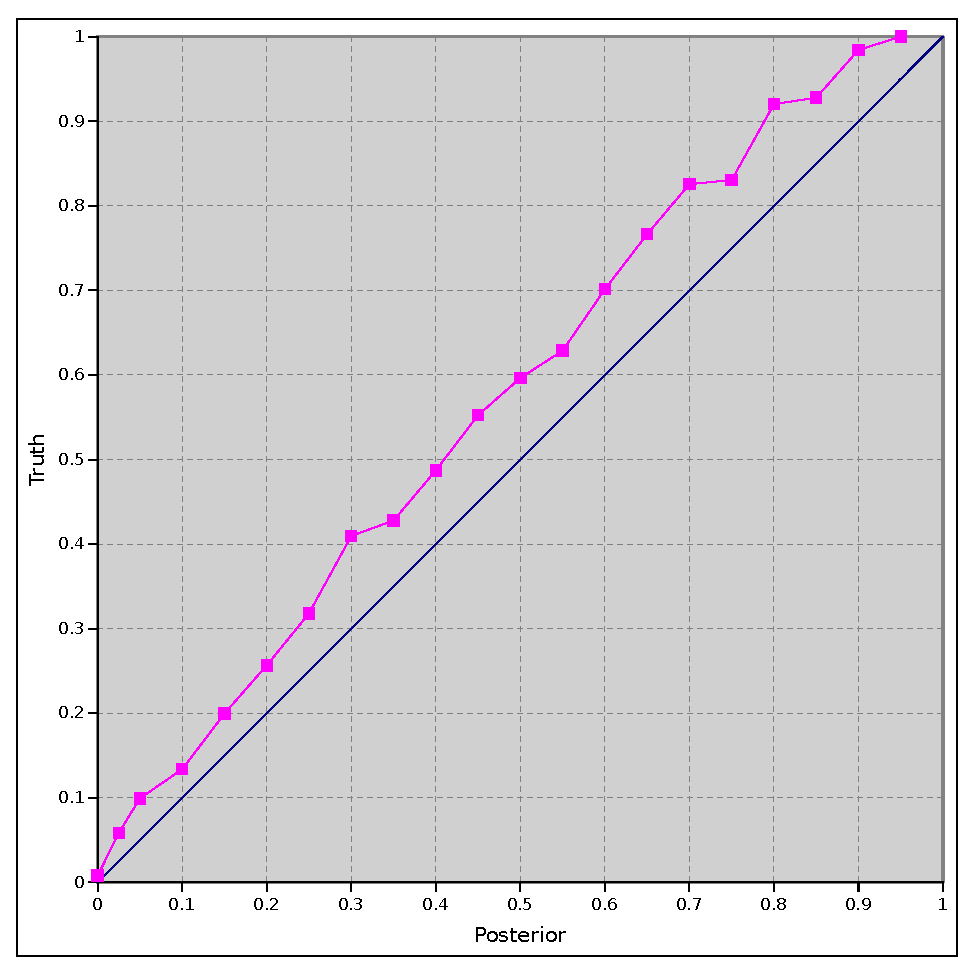
\includegraphics[width=\textwidth]{direction_platonic_58}
  \caption{Simulated data using 10k each chain and collide models with
    flatly random parameters, using 0.05-sized buckets for the
    posterior.  Higher numbers indicate collider.}
  \label{dir_pla58}
\end{figure}

\begin{figure}
  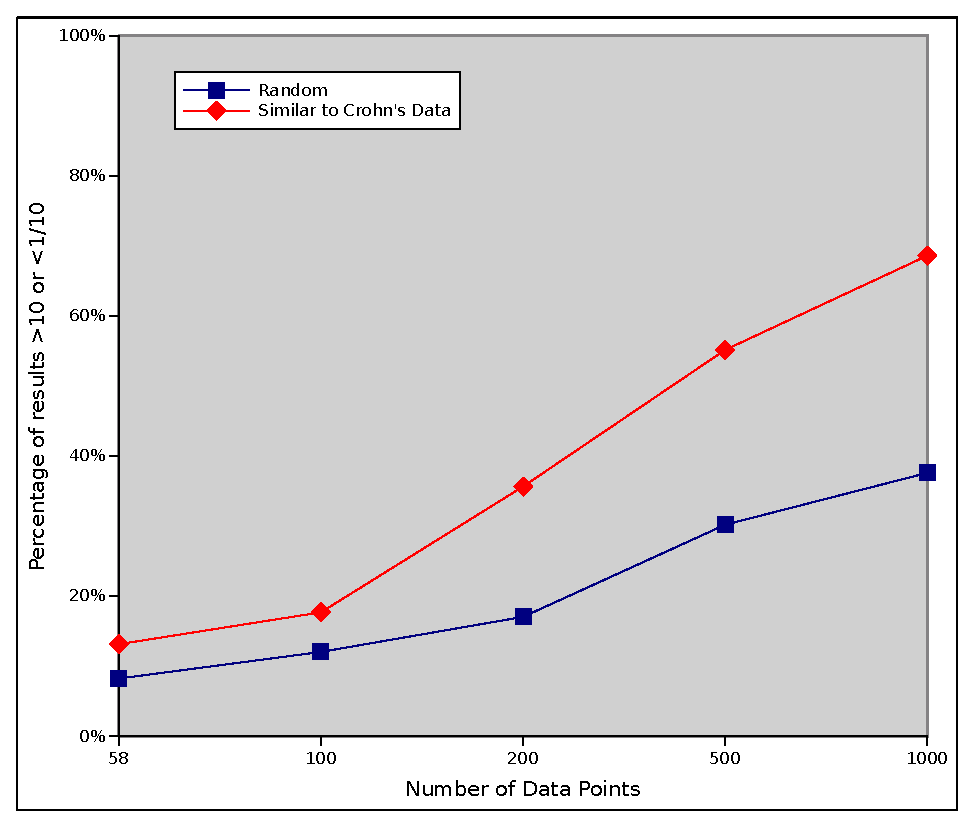
\includegraphics[width=\textwidth]{usefullness}
  \caption{Fraction of bayes factors that were at least 10:1 one way
    or the other as a function of dataset size}
  \label{dir_use}
\end{figure}

\begin{figure}
  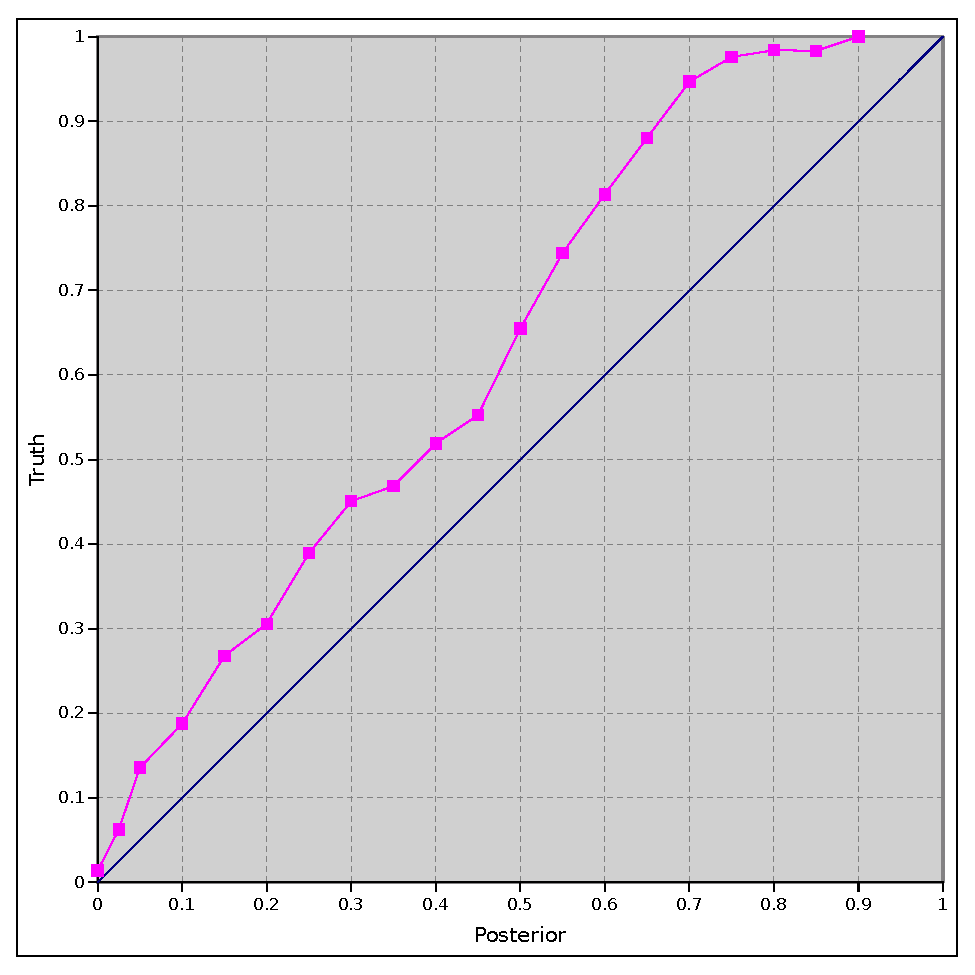
\includegraphics[width=\textwidth]{direction_crohns_58}
  \caption{The same simulation as \ref{dir_pla58}, but with p(NOD2) and
    p(ICD$|$NOD2) taken from data, and the independences measurable by
    $\chi^2$ test.}
  \label{dir_crohns58}
\end{figure}

\begin{figure}
  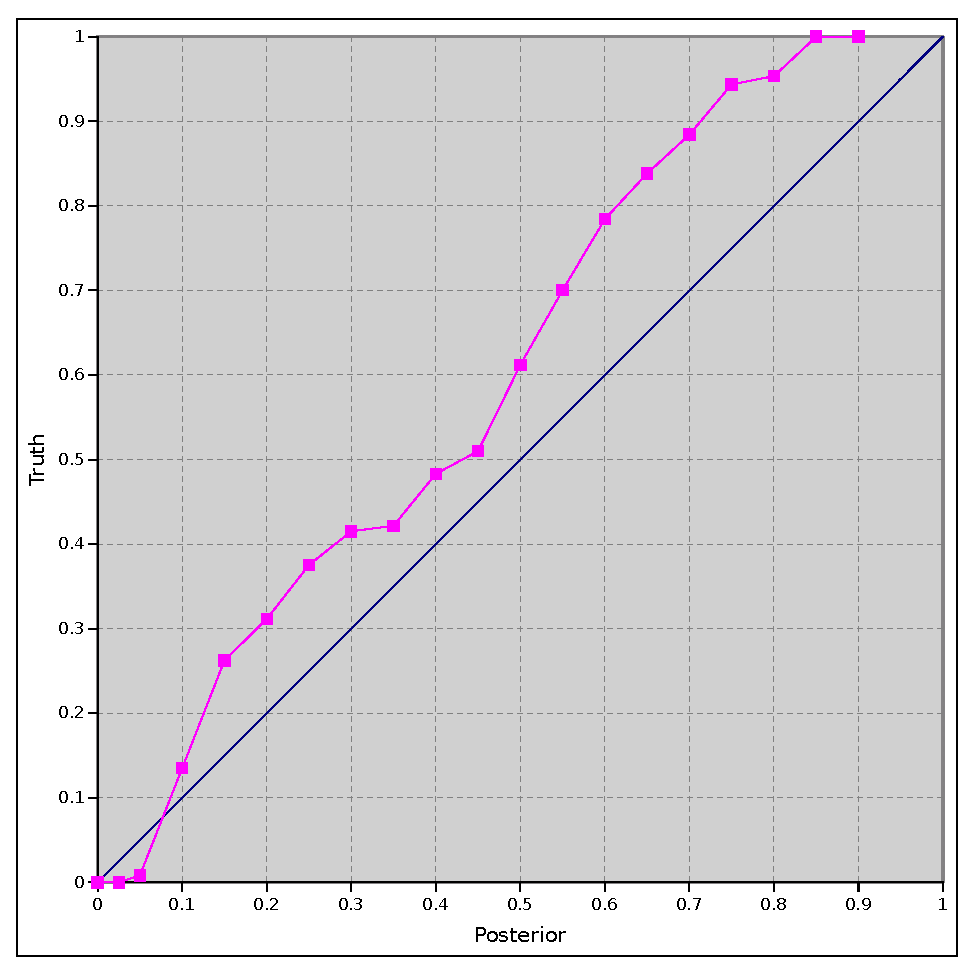
\includegraphics[width=\textwidth]{direction_multi_58}
  \caption{The same simulation as \ref{dir_crohns58}, but with
    allowing an $A\rightarrow C$ causal link, albeit one which does
    not show up as $A\not\indep C$ on a $\chi^2$ test.}
  \label{dir_multi58}
\end{figure}

\begin{figure}
  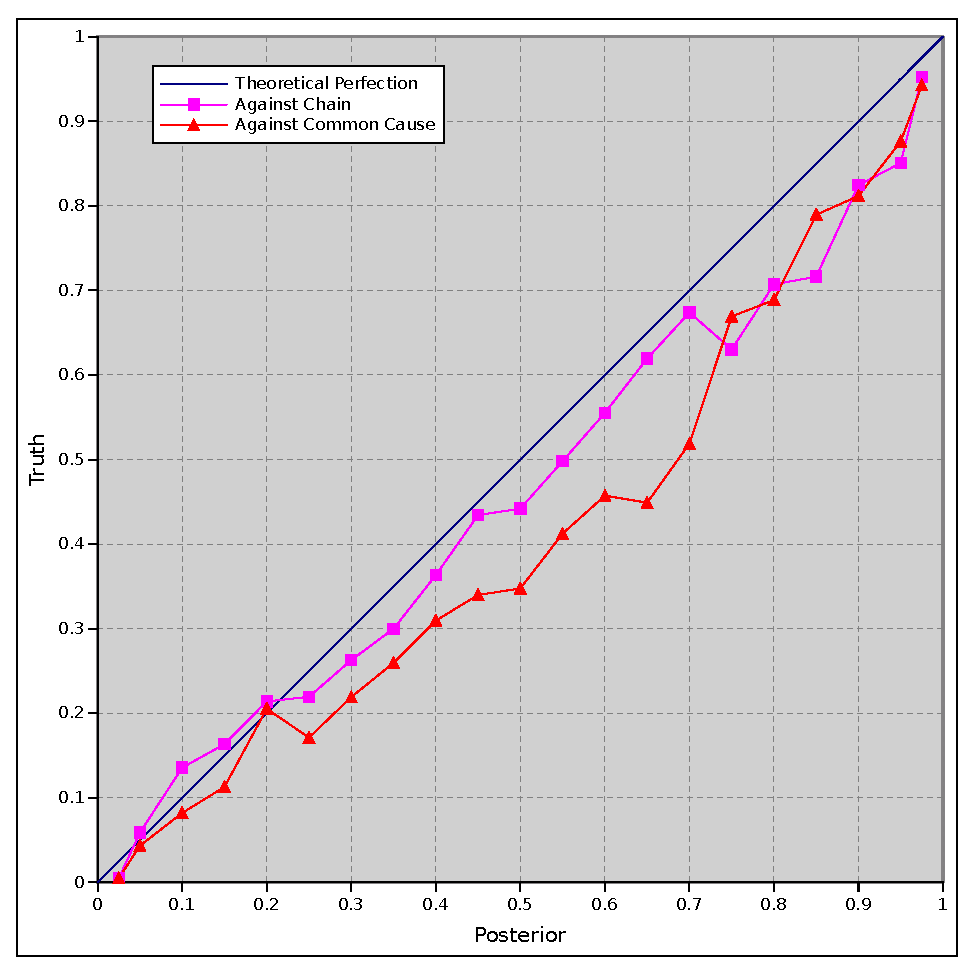
\includegraphics[width=\textwidth]{sever}
  \caption{Calibration for the severing test, both in the case it was
    designed for and in the case of comparing severing to common
    cause.  Higher probabilities indicate severing.}
  \label{sever}
\end{figure}

\begin{figure}
  \begin{tabular}{llrr}
    Species & Sick When & P-Value ICD link & Bayes Factor Causality \\
    Streptococcus pseudopneumoniae & $>$6.36E-05 & 3.1e-05 & 5.15 \\
    Streptococcus infantis & present & 0.0014 & 2.55 \\
    Lactobacillus acidophilus & $>$8.15E-05 & 0.00017 & 10.64 \\
    Sphingopyxis alaskensis & present & 0.0004 & 2.43 \\
    Clostridium methylpentosum & $\leq$6.31E-04 & 0.00085 & 2.53 \\
    Roseiflexus castenholzii & present & 7.3e-05 & 3.30 \\
    Ruminococcus faecis & $\leq$1.07E-03 & 0.0022 & 2.40 \\
  \end{tabular}
  \caption{Results of the direction test on 222 interesting species,
    using $\chi^2$ to check a relationship to Crohn's Disease and the
    direction test described here to establish that it causes (or
    prevents) the disease.}
  \label{dir_tab}
\end{figure}

\end{document}
